
\begin{figure}[H]
	\centering
	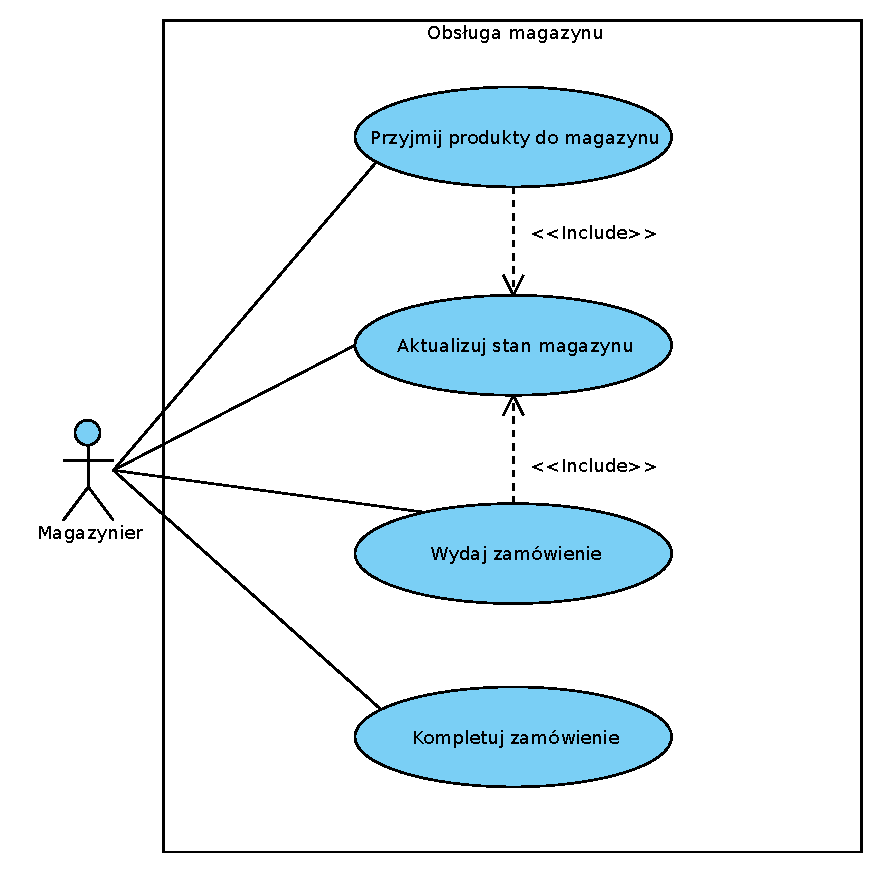
\includegraphics[width=.8\textwidth]{img/UC/magazyn.eps}
\end{figure}

\textbf{Numer i Nazwa przypadku użycia:} UC01 - Przyjmij produkty do magazynu \\
\textbf{Autor:} Magazynier\\
\textbf{Cel przypadku użycia:} Dodanie produktów recyklingu do magazynu i aktualizacja stanu magazynu \\
\textbf{Kontekst użycia:} przechowanie produktów recyklingu w magazynie\\
\textbf{Zakres:} system magazynowy \\
\textbf{Poziom:} biznesowy \\
\textbf{Aktor główny:} Magazynier \\
\textbf{Uczestnicy:} Kierowca \\
\textbf{Wyzwalacz:} dostarczenie przez kierowce produktów do magazynu \\
\textbf{Warunek początkowy:} kierowca ma produkty recyklingu, które należy zmagazynować oraz ich listę \\
\textbf{Minimalna gwarancja:} w przypadku, gdy produkty nie zostaną zmagazynowane, stan magazynu nie będzie zmieniany \\
\textbf{Główny scenariusz powodzenia:} \\
	\begin{enumerate}
		\item Kierowca przywozi produkty
		\item Magazynier układa je w magazynie
		\item Magazynier aktualizuje stan magazynu
	\end{enumerate}
\begin{figure}[H]
	\centering
	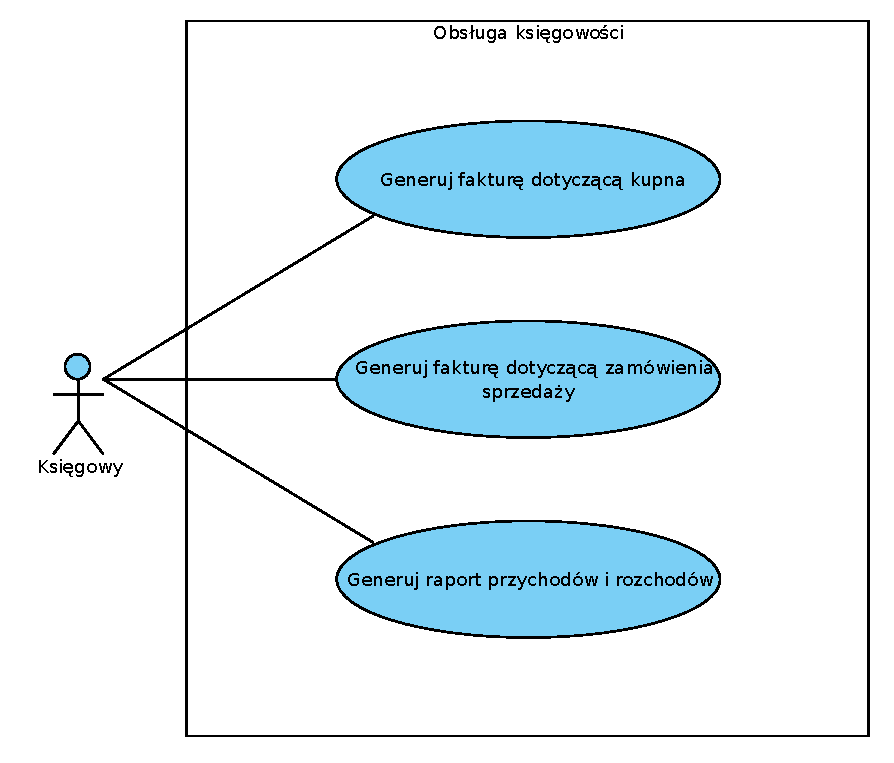
\includegraphics[width=.8\textwidth]{img/UC/ksiegowosc.eps}
\end{figure}

\textbf{Numer i Nazwa przypadku użycia:} UC02 - Wydaj zamówienie \\
\textbf{Autor:} Magazynier\\
\textbf{Cel przypadku użycia:} Wydanie kierowcy produktów, ujętych w zamówieniu \\
\textbf{Kontekst użycia:} potrzeba przetransporotowania produktów do kupca\\
\textbf{Zakres:} system magazynowy \\
\textbf{Poziom:} biznesowy \\
\textbf{Aktor główny:} Magazynier \\
\textbf{Uczestnicy:} Kierowca \\
\textbf{Wyzwalacz:} przyjazd kierowcy do magazynu \\
\textbf{Warunek początkowy:} kierowca ma zamówienie \\
\textbf{Minimalna gwarancja:} w przypadku, gdy nie można skompletować zamówienia stan magazynu się nie zmieni \\
\textbf{Główny scenariusz powodzenia:} \\
	\begin{enumerate}
		\item Kierowca przekazuje numer zamówienia magazynierowi
		\item Magazynier wydaje produkty kierowcy
		\item Magazynier uaktualnia stan magazynu
	\end{enumerate}
\textbf{Rozszerzenia:} \\
1.1 W przypadku gdy magazynier nie otrzymał wcześniej informacji o zamówieniu, kompletuje je teraz, w razie niepowodzenia produkty nie zostają wydane\\

\textbf{Numer i Nazwa przypadku użycia:} UC03 - Aktualizuj stan magazynu \\
\textbf{Autor:} Magazynier\\
\textbf{Cel przypadku użycia:} Aktualizacja danych o stanie magayznu \\
\textbf{Kontekst użycia:} utrzymywanie aktualnej informacji o ilości produktów w magazynie \\
\textbf{Zakres:} system magazynowy \\
\textbf{Poziom:} użytkowy \\
\textbf{Aktor główny:} Magazynier \\
\textbf{Wyzwalacz:} wydanie lub przyjęcie produktów \\
\textbf{Warunek początkowy:} zmiana stanu magazynu \\
\textbf{Minimalna gwarancja:} w przypadku, gdy nie można zaktualizować stanu magazynu, jego stan pozostanie niezmieniony \\
\textbf{Główny scenariusz powodzenia:} \\
	\begin{enumerate}
		\item Magazynier wpisuje informację o wydanych/przyjętych produktach
	\end{enumerate}

\textbf{Numer i Nazwa przypadku użycia:} UC04 - Kompletuj zamówienie \\
\textbf{Autor:} Magazynier\\
\textbf{Cel przypadku użycia:} Skompletowanie zamówienie w celu wydania go kierowcy \\
\textbf{Kontekst użycia:} chęć uporządkowania produktów do zamówienia w celu szybkiego ich przekazania kierowcy \\
\textbf{Zakres:} system magazynowy \\
\textbf{Poziom:} biznesowy \\
\textbf{Aktor główny:} Magazynier \\
\textbf{Wyzwalacz:} dostanie informacji o zamówieniu \\
\textbf{Warunek początkowy:} odpowiednia ilość towarów w magazynie \\
\textbf{Minimalna gwarancja:} w przypadku, gdy nie ma odpowiedniej ilości towarów w magazynie, zostanie wysłana informacja zwrotna  \\
\textbf{Główny scenariusz powodzenia:} \\
	\begin{enumerate}
		\item Magazynier otrzymuje listę towarów, które wchodzą w skład zamówienia
		\item Magazynier sprawdza czy posiada ich odpowiednią ilość
		\item Magazynier przygotowuje zamówienie
	\end{enumerate}
\textbf{Rozszerzenia:} \\
2.1. Nie można skompletować zamówienia, zostaje wysłana informacja zwrotna o nieposiadanych towarach\\

\begin{figure}[H]
	\centering
	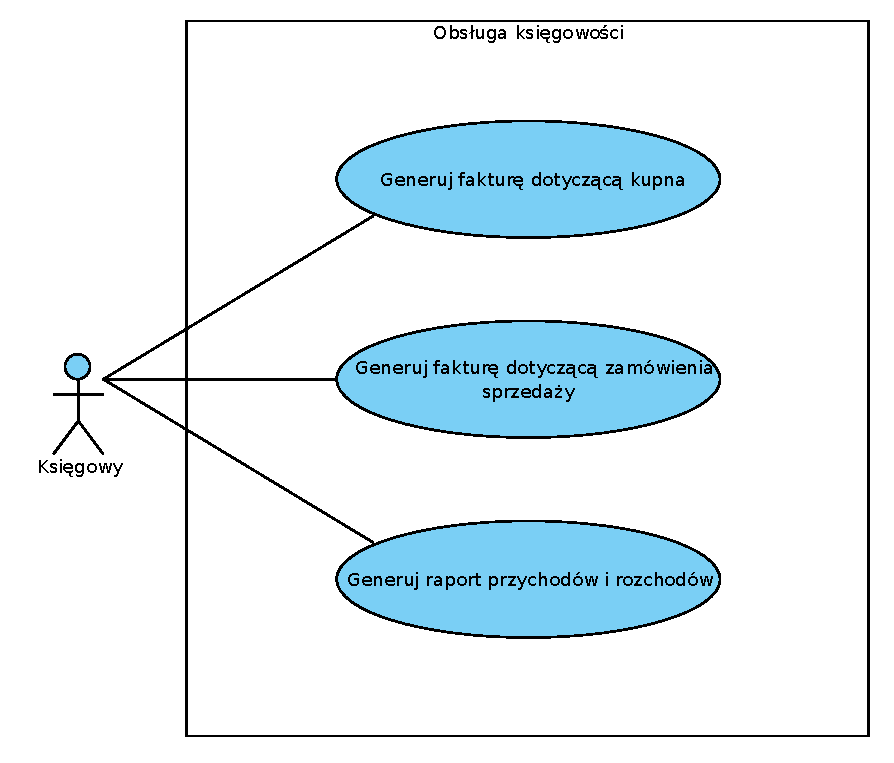
\includegraphics[width=.8\textwidth]{img/UC/ksiegowosc.eps}
\end{figure}
\begin{figure}[H]
	\centering
	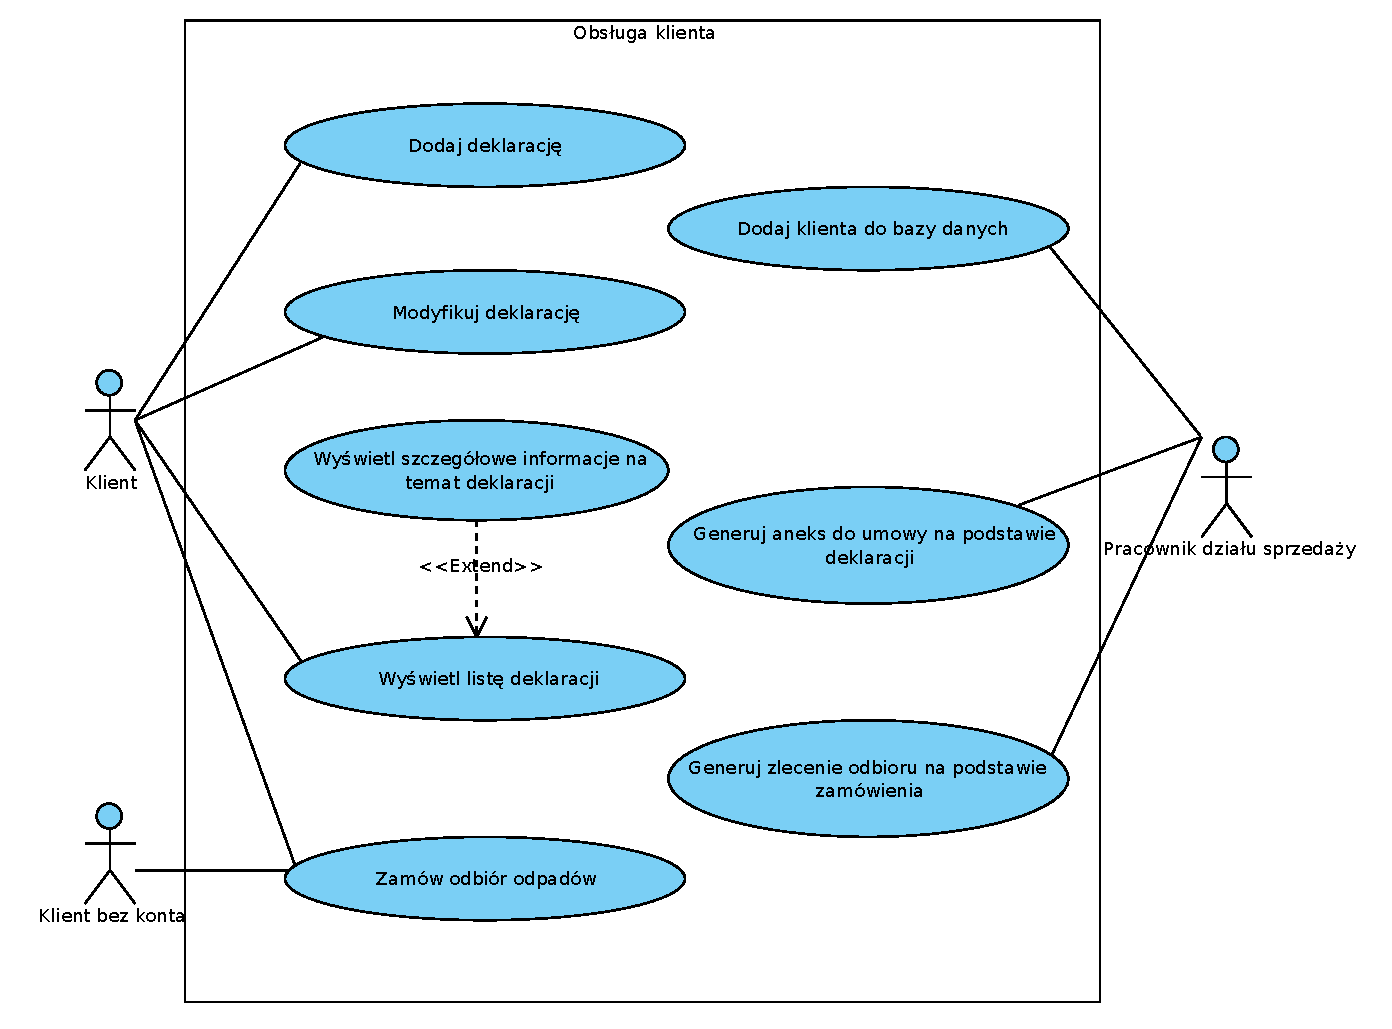
\includegraphics[width=1.1\textwidth]{img/UC/deklaracje.eps}
\end{figure}